\documentclass{article}
\usepackage{iclr2027_conference,times}
\input{math_commands.tex}
\usepackage{hyperref}
\usepackage{url}
\usepackage{booktabs}
\usepackage{amsmath,amssymb}
\usepackage{graphicx}
\usepackage{microtype}
\usepackage{xcolor}

\title{Does the Benchmark Require the Input?\\Falsification Audits for Structured Agent Evaluation}
\author{Anonymous authors}

\newcommand{\casepath}{\textsc{CasePath}}
\newcommand{\const}{\textsc{Constant}}
\newcommand{\excess}{\operatorname{Excess}}

\begin{document}
\maketitle
\begin{abstract}
Structured agents are often evaluated with metrics interpreted as evidence that they use an explicit representation to respond to the current instance. We ask a prior question: \emph{does the benchmark require the input at all?} We operationalize three falsification tests: a scenario-cross-fitted input-independent oracle, a permutation that reassigns outputs to the wrong inputs, and evaluator-independence checks. For a set-retraction metric we also derive the optimal fixed withdrawal policy in closed form under a volume-matched chance correction. On two independently constructed source-grounded legal workflow scopes, the static task has one observed gold checklist and a case-ignoring F1 of 1.000. A paired intervention task designed specifically to escape that degeneracy fails again: cross-fitted constant policies obtain excess withdrawal recall of $+0.447$ and $+0.752$, versus $+0.118$ and $+0.018$ for the strongest measured agents. Within-scenario output--label permutations leave the apparent leading behavior ordinary or invariant. A preregistered robustness study with three non-OpenAI evaluator families (522 calls) shows that changing the evaluator does not rescue the benchmark: Claude Opus 5 reproduces all 58 reference document sets and all 28 paired release sets exactly, and a family-balanced consensus agrees exactly on every complete common pair. The conclusion is therefore not that one agent fails, but that these evaluations do not identify case-conditioned competence. We release the falsification audit and the full negative record as a reproducible benchmark-validity test.
\end{abstract}

\section{Introduction}
A benchmark score is normally read as evidence about a system: the model understood the passage, the agent used its plan, or the structured representation helped on the current instance. That interpretation requires more than a high number. The score must depend on the information the claim says the system used.

This requirement is easy to violate. Partial-input baselines have exposed annotation artifacts in reading comprehension and natural-language inference \citep{kaushik2018reading,poliak2018hypothesis,gururangan2018artifacts}; shortcut learning more generally describes decision rules that score well without implementing the intended behavior \citep{geirhos2020shortcut}. Recent work makes the broader point in terms of evaluation validity and metric misspecification \citep{thomas2026validity,joshi2026guardians}. Yet structured-agent evaluations increasingly add plans, graphs, tools, judges, and multi-stage metrics, creating more ways for a score to look causal while remaining insensitive to the instance.
We encountered this failure twice while building \casepath, a source-grounded agent that maps authoritative passages to propositions, process nodes, evidence capabilities, and document requirements. The first benchmark was static: predict which documents a case requires. We discovered that every measured case in each of two scopes had the same gold checklist. We therefore replaced the static task with paired interventions: add one branch-settling fact to the same case and score which now-unnecessary documents the agent retracts. The paired design was intended to remove the constant level that saturated the static task. It did not. A policy that never reads the case is dramatically stronger than every measured system on both scopes.

That failure is scientifically useful because it survived controls that initially looked reassuring. The paired task had a frozen scenario split, a preregistration, a per-arm volume correction, scenario-cluster bootstrap intervals, and four interpreter models. Several cells were far from zero. None of those checks asked whether the score changed when outputs were attached to the wrong cases or whether a fixed policy could do better. Once we ask those questions, the headline disappears.

We make three contributions. First, we give an executable \emph{input-dependence audit}: cross-fit the strongest constant policy across groups, permute output--target pairings while preserving groups, and report both beside the system. For our set-retraction metric, the optimal fixed withdrawal set has a closed-form threshold. Second, we show that the failure replicates across two independently authored workflow contracts: a constant policy beats the strongest measured agent by $3.8\times$ on rent increase and by more than $40\times$ on termination. Third, we separate benchmark degeneracy from evaluator leakage. A preregistered 522-call study with Claude Opus 5, Gemini 3.1 Pro, and DeepSeek V4 Pro independently reconstructs the reference states. The benchmark conclusions remain unchanged; on full-coverage Opus judgments, every reference document set and every release set matches the original evaluator exactly.

Our claim is deliberately narrower than ``structured agents do not work.'' We show that these two benchmark instances do not identify case-conditioned retraction. The representation may still be useful; this evaluation cannot establish that. This distinction matters especially in expert domains, where attractive benchmark numbers can be mistaken for evidence of real workflow competence \citep{medvedeva2023right,lou2026lawyering}.
\section{Related Work}
\paragraph{Input-free and shortcut baselines.}
Hypothesis-only and passage-only baselines established a simple diagnostic principle: if the task claims that prediction requires two inputs, evaluate a model that removes one of them \citep{kaushik2018reading,poliak2018hypothesis,gururangan2018artifacts}. Annotation artifacts can make such degenerate models surprisingly competitive \citep{poliak2018hypothesis,gururangan2018artifacts}. Shortcut learning generalizes this observation to high-performing decision rules that exploit unintended regularities \citep{geirhos2020shortcut}; recent LLM studies show that scale does not eliminate shortcut use \citep{yuan2024shortcut}. Our setting differs in two ways. The output is a changing \emph{set} rather than a class, and the benchmark was itself redesigned as a paired intervention after a static shortcut was discovered. We therefore need an input-independent oracle for a change metric, not merely a majority label.

\paragraph{Adversarial acceptance checks for agent benchmarks.}
Contemporaneous agent-evaluation work already treats a passing oracle as insufficient. ATLAS includes no-op, scripted-cheater, determinism, and seed-generalization checks \citep{arcifa2026atlas}; Terminal-Bench 3 similarly runs no-op validation and adversarial cheat trials during task review \citep{terminalbench3review}. We build on this principle rather than claim no-op testing as new. Our failure is subtler: a literal no-op need not score, yet an optimized policy that never reads the instance can dominate a paired, volume-corrected set-change metric. Cross-fitting makes that shortcut an out-of-group baseline, and wrong-pairing permutations test instance dependence even when outputs are not constant.

\paragraph{Evaluation validity and identifiability.}
\citet{thomas2026validity} argue that an evaluation is useful only to the extent that its metric represents the phenomenon of interest. \citet{joshi2026guardians} show a related failure in representation learning: standard metrics can produce false positives and negatives when their structural assumptions are violated. We operationalize this perspective for agentic, set-valued workflows. Rather than infer validity from metric semantics, we try to falsify an input-conditioned interpretation directly: remove the input, break its pairing to the target, and vary the evaluator.

\paragraph{Evaluator dependence.}
LLM-based evaluators can favor related generators or model families; \citet{li2026preference} call this preference leakage. Our original reference adjudicator was also one of the interpreter models under test, so this is a live confound rather than a hypothetical one. We therefore freeze an independent three-family adjudication study before execution and report both the full per-family matrix and a family-balanced consensus. The robustness result reduces this confound but does not repair a benchmark that an input-free policy already wins.

\paragraph{Legal benchmark validity.}
Legal-AI work has independently emphasized that benchmark labels and inputs may fail to represent the professional task being claimed \citep{medvedeva2023right,lou2026lawyering}. We use Swiss tenancy workflows only as a demanding case study; the proposed falsifiers are domain-agnostic and operate on the benchmark's predictions and targets rather than on legal doctrine.
\section{Falsifying an Input-Conditioned Evaluation Claim}
Consider paired instances $(x_i,x_i')$. A reference evaluator maps them to required-document sets $R_i$ and $R_i'$, with gold release set $E_i=R_i\setminus R_i'$. A system produces request sets $B_i$ before and $A_i$ after the intervention; its withdrawal is $W_i=B_i\setminus A_i$. Raw withdrawal recall is $\sum_i|W_i\cap E_i|/\sum_i|E_i|$.

A system that requests more documents has more opportunities to withdraw a correct one. We therefore compare each system to itself withdrawing the same number of its own requested documents uniformly at random. Conditional on $(B_i,W_i,E_i)$, the expected random hits are exactly
\begin{equation}
  \E |W_i^{\rm rand}\cap E_i| = |W_i|\frac{|B_i\cap E_i|}{|B_i|},
\end{equation}
with zero when $B_i$ is empty. The reported volume-corrected statistic is
\begin{equation}
\excess = \frac{\sum_i |W_i\cap E_i|-\sum_i |W_i| |B_i\cap E_i|/|B_i|}{\sum_i|E_i|}.
\label{eq:excess}
\end{equation}
This chance correction is useful but insufficient: it controls \emph{how many} documents are withdrawn, not whether the choice was computed from this input.

\subsection{Audit 1: the strongest input-independent constant}
Let a constant policy request a fixed set $B$ and withdraw a fixed $W\subseteq B$ for every pair. Define $f_d=\sum_i\mathbf{1}[d\in E_i]$ and $C=\sum_i|B\cap E_i|$. Substituting the constant policy into Eq.~\ref{eq:excess} makes its numerator
\begin{equation}
 \sum_{d\in W}\left(f_d-\frac{C}{|B|}\right).
\end{equation}
The optimal fixed withdrawal is therefore available in closed form:
\begin{equation}
 W^*(B)=\left\{d\in B: f_d>\frac{C}{|B|}\right\}.
 \label{eq:constant}
\end{equation}
We take $B$ to be the modal pre-intervention reference set on training groups. To avoid an in-sample oracle, we leave out one scenario at a time, derive $(B,W^*)$ from the remaining scenarios, and evaluate it only on the held-out scenario. A claimed case-sensitive system should outperform this cross-fitted policy, which never receives $x_i$.
\subsection{Audit 2: pairing sensitivity}
Even a non-constant system can score well for the wrong reason if target regularities dominate instance-specific information. We therefore hold every system output $(B_i,W_i)$ fixed and randomly permute the release sets $E_i$ across pairs, recomputing Eq.~\ref{eq:excess}. We report both unrestricted permutations and the stricter null that permutes only within scenario. The latter preserves group composition and asks whether the system output is paired to the \emph{right case within the same scenario}. If the observed statistic is ordinary under this wrong-pairing null, the score does not demonstrate case-specific information.

\subsection{Audit 3: evaluator independence}
When targets are model-adjudicated, a system score is potentially a function of the evaluator as well as the system. We therefore freeze a second reference construction before inspecting any new judgments. Three non-OpenAI model families independently receive the original reference prompt, contract, and 58 rent-increase narratives, with three temperature-zero calls per unit. We aggregate within family and then equally across families. Unparseable semantic outputs are retained as failures and never rerun; a family requires at least two valid calls for a unit, and the three-family consensus requires all three family-level judgments. We report reference-set agreement, release-set agreement, and the complete interpreter-by-evaluator score matrix.

These audits are falsifiers, not sufficient conditions for real-world validity. Passing them says only that the easiest input-independence explanations did not survive. Failing either of the first two is stronger: the benchmark cannot support an input-conditioned interpretation of the reported score.

\section{Case Study: Source-Grounded Workflow Retraction}
\subsection{System and data}
\casepath is a local source-grounded workflow agent. It fetches consolidated Swiss federal law, extracts operational propositions whose cited spans must occur verbatim in the source, induces a process graph, resolves branch predicates against a case narrative, maps active obligations to required facts and evidence capabilities, and routes those capabilities to a fixed document catalogue. The checklist is compiled deterministically from the active graph. A document is released only when no active node still requires it. These mechanics motivate a natural claim: an explicit process representation should support coherent retraction when a new fact settles a branch.

We evaluate two separately authored tenancy scopes over a synthetic 150-claim intake corpus: rent increase and termination. No real claim is used. Rent increase contributes 30 held-out originals and 28 complete paired interventions over six scenarios; termination contributes 49 pairs over eight scenarios. Scenario, not surface wording or language twin, is the resampling and cross-fitting unit. The reference contracts are authored separately from the induced graph and map open decisions to document requirements. The operational document-layer capacities---the number of distinct unions expressible by arbitrary open/closed decision masks---are 13 for rent increase and 672 for termination. We call this \emph{capacity}, not legal reachability: arbitrary masks need not correspond to legally reachable states.
\subsection{Arms, interpreters, and scoring}
The main rent-increase comparison uses three matched arms: \texttt{b1\_direct}, which predicts the checklist directly; \texttt{b3\_graph\_then\_list}, which sees the induced graph as context but predicts the list; and \texttt{b5\_induced\_graph}, which interprets branch predicates and then deterministically compiles the active graph. The model-generality study reruns \texttt{b1} and \texttt{b5} with GPT-5.6 Terra, Claude Haiku 4.5, Gemini 2.5 Flash, and DeepSeek v3.2, holding graph, contract, cases, catalogue, temperature, token limit, and code fixed. Termination uses the same three-arm structure with its own independently authored graph and contract.

All headline intervals resample scenarios with 5,000 cluster-bootstrap draws. Pairing tests use 5,000 permutations. The volume baseline is the exact hypergeometric expectation in Eq.~\ref{eq:excess}, not a Monte Carlo approximation. Historical runners are bound to artifact hashes, runner hashes, model identity, temperature and token settings in a machine-readable sidecar. Final successful outputs exist for every historical interpreter unit; the old runners did not preserve a complete transient retry/error ledger, which we treat as a reproducibility limitation rather than infer away.

\subsection{Why this became a validity study}
The original static task asked which documents each case required. Both scopes unexpectedly produced one observed gold checklist across all measured cases. We therefore built the paired intervention task to score \emph{change}, reasoning that differencing would remove the constant level. The paired experiment was preregistered and executed before the input-independence audit in this paper. The audit was prompted by hostile review of the resulting positive-looking cells. We preserve that sequence because it is precisely the failure mode the paper studies: a seemingly stronger experimental design can inherit the same shortcut at a different level.

\section{Results}
\subsection{Static and paired tasks both fail the input-dependence test}
Table~\ref{tab:core} summarizes the central result. Despite document-layer capacities of 13 and 672, respectively, rent increase and termination each have exactly one observed static gold checklist. The case-ignoring static oracle therefore obtains F1 1.000 on both scopes.

\begin{table}[t]
\centering
\caption{The benchmark does not require the case. ``Capacity'' is the number of distinct document unions expressible by arbitrary decision masks; ``gold sets'' is the number observed in the corpus. Dynamic values are Eq.~\ref{eq:excess}.}
\label{tab:core}
\resizebox{\linewidth}{!}{\begin{tabular}{lrrrrrr}
\toprule
Scope & Pairs & Gold sets & No-input $\mu$F1 & Best agent $\mu$F1 & No-input exact & Best agent exact \\
\midrule
Rent increase & 28 & 3 & 0.919 & 0.459 & 0.643 & 0.071 \\
Termination & 49 & 4 & 0.589 & 0.078 & 0.551 & 0.531 \\
\bottomrule
\end{tabular}
}
\end{table}
The paired task is more deceptive. On rent increase, the cross-fitted constant requests the same ten-document pre-intervention checklist and withdraws the same five documents in every fold. It achieves raw withdrawal recall 0.947. After its own exact volume baseline of 0.500, excess is $+0.447$ with 95\% scenario-bootstrap interval $[+0.429,+0.475]$. The strongest measured agent reaches only $+0.118$ $[+0.107,+0.125]$.

Termination is an independent replication and a stricter test because the most common individual release set is empty. The cross-fitted optimization in Eq.~\ref{eq:constant} nevertheless recovers the same non-empty fixed policy in all eight folds: request the constant 17-document checklist and always withdraw \texttt{bank\_statement}, \texttt{extension\_request}, \texttt{payment\_deadline\_warning\_letter}, and \texttt{rent\_payment\_records}. It obtains raw recall 0.987, random baseline 0.235, and excess $+0.752$ $[+0.728,+0.765]$. The strongest measured agent is $+0.018$ with an interval spanning zero. Thus the failure is not specific to a modal-release heuristic or to one contract.

\begin{figure}[t]
  \centering
  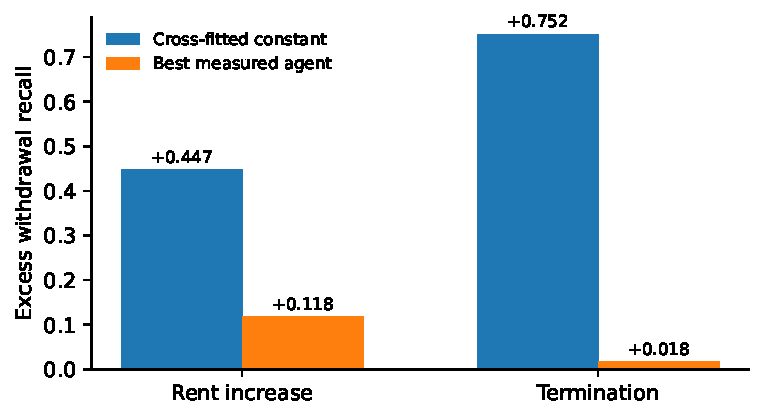
\includegraphics[width=.95\linewidth]{fig_constant_vs_agent.pdf}
  \caption{Scenario-cross-fitted policies that never read the case outperform the strongest measured agent on both dynamic scopes. Values are volume-corrected excess withdrawal recall.}
  \label{fig:constant}
\end{figure}

A corrupted long-narrative scenario is not responsible for the rent result. Removing \texttt{S8\_nebenkosten\_reclass} entirely leaves 24 pairs; the cross-fitted constant remains $+0.445$ $[+0.426,+0.473]$, while \texttt{b5} remains $+0.118$ $[+0.106,+0.125]$.

\subsection{Wrong case-to-label pairings reproduce the apparent agent effects}
The second falsifier asks whether the score knows \emph{which case} produced an output. For rent increase, every \texttt{b5} interpreter lies inside its within-scenario wrong-pairing null. GPT's observed $+0.118$ has $p=0.75$ under within-scenario permutations; Gemini's $+0.108$ is exactly invariant to reassignment; Claude Haiku and DeepSeek have $p=1.00$ and $p\approx0.60$, respectively. The four \texttt{b5} conditions emit only 1, 2, 1, and 1 distinct pre-intervention request sets across 28 pairs. Their score differences are therefore mostly differences among standing document habits, not evidence of case-conditioned retraction.

\begin{figure}[t]
  \centering
  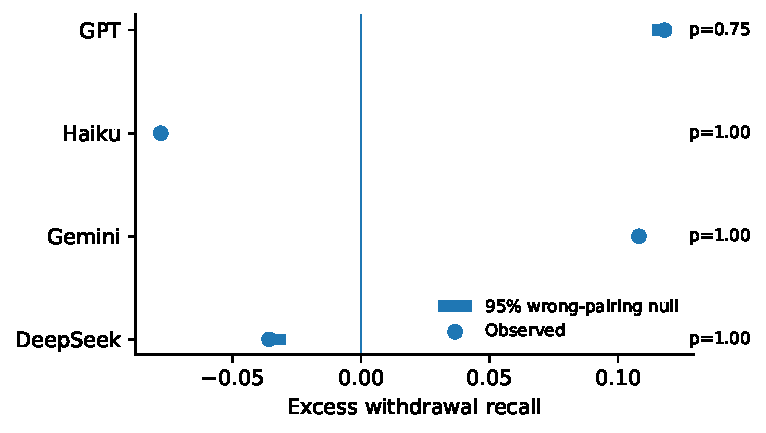
\includegraphics[width=.95\linewidth]{fig_pairing_null.pdf}
  \caption{Observed rent-increase \texttt{b5} scores (points) against 95\% within-scenario wrong-pairing null ranges (bars). None clears the null.}
  \label{fig:perm}
\end{figure}
\subsection{Independent evaluators do not rescue the benchmark}
The original reference was authored by GPT-5.6 Terra, creating a serious evaluator-relatedness concern \citep{li2026preference}. We therefore froze and executed a 522-call study before reading the new judgments. Claude Opus 5 produced valid family-level adjudications for all 58 units, Gemini 3.1 Pro for 51, and DeepSeek V4 Pro for 50. The conservative family-balanced consensus requires all three and covers 43 units, yielding 17 complete intervention pairs.

The result reduces the evaluator-confound rather than explaining the degeneracy. Opus reproduces the original reference document set on 58/58 units and the release set on 28/28 paired units exactly. Gemini does so on 51/51 units and 23/23 complete pairs. DeepSeek agrees on 92\% of reference document sets and 82\% of its 22 complete release pairs. The three-family consensus agrees exactly with the original reference on all 43 complete common units and all 17 complete common pairs. Table~\ref{tab:evaluator} shows that the input-independent oracle remains roughly four times the strongest agent under every evaluator.

\begin{table}[t]
\centering
\caption{Evaluator robustness on rent increase. ``Agreement'' is exact release-set agreement with the original GPT reference on the available paired subset. The three-family consensus is complete-case and therefore conservative.}
\label{tab:evaluator}
\resizebox{\linewidth}{!}{\begin{tabular}{lrrr}
\toprule
Evaluator & Complete pairs & Exact release agreement & GPT-B5 excess \\
\midrule
GPT-5.6 Terra & 28 & -- & +0.118 \\
Claude Opus 5 & 28 & 100.0\% & +0.118 \\
Gemini 3.1 Pro & 23 & 100.0\% & +0.118 \\
DeepSeek V4 Pro & 22 & 81.8\% & +0.115 \\
3-family consensus & 17 & 100.0\% & +0.116 \\
\bottomrule
\end{tabular}
}
\end{table}

On the common 17-pair consensus subset, switching from the original GPT reference to the external family-balanced reference changes each interpreter's excess by exactly 0.000 under the frozen analysis. The interpreter ordering also remains GPT ($+0.116$), Gemini ($+0.106$), DeepSeek ($-0.038$), Haiku ($-0.072$). This does \emph{not} rehabilitate the metric: the cross-fitted constant on the same consensus reference is $+0.430$.

The evaluator study also exposes a useful distinction between decision-state agreement and benchmark-output agreement. Opus agrees with the original GPT decision status on only 45.5\% of decision comparisons, yet the induced document sets agree 100\%. Many decision disagreements are therefore invisible after unioning document requirements. The benchmark output is more invariant than the underlying adjudication, another reason not to infer rich process understanding from the set score alone.

\subsection{Why the earlier controls looked convincing}
The original uncontrolled comparison made the compiled arm appear $+0.553$ better than direct prediction in withdrawal recall. A post hoc but necessary volume control reduces the compiled arm to $+0.118$: roughly four fifths of its raw recall is reproduced by withdrawing the same number of its own requested documents at random. Direct prediction even moves below its own baseline on the original GPT condition. However, Eq.~\ref{eq:excess} still rewards a fixed preference over document types whenever the gold release set is concentrated. The cross-fitted constant and pairing permutation are therefore complementary to volume correction, not replacements for it.

Changing the interpreter while freezing the representation also produces large score changes: the same \texttt{b5} artifact is $+0.118$ with GPT, $+0.108$ with Gemini, $-0.036$ with DeepSeek and $-0.078$ with Haiku. We do not interpret these as four estimates of ``retraction ability'': the permutation audit shows the conditions are near-constant functions of the case. What they establish is the narrower attribution point that a structured representation is not self-executing; a score from representation $R$ interpreted by model $M$ is a property of the pair $(R,M)$ unless an interaction study shows otherwise.
\section{A Minimal Validity Audit for Structured-Agent Benchmarks}
The empirical lesson is not to add one more baseline after results are known, but to make input dependence an admission criterion for the benchmark. We recommend reporting four quantities before attributing a task score to structured reasoning.

\paragraph{1. Input-independent ceiling.}
Train the strongest constant policy that is allowed to use the training labels but never the evaluation input, and evaluate it out of group. For set-valued retraction under Eq.~\ref{eq:excess}, Eq.~\ref{eq:constant} makes this a closed-form calculation. For other metrics, the oracle may be a learned bias-only model or empirical-risk-minimizing constant. The key is to optimize the shortcut fairly rather than compare against an arbitrarily weak majority baseline.

\paragraph{2. Pairing permutation.}
Reassign targets across system outputs, preferably within the highest-level grouping used for inference. If the observed statistic is typical when evaluated against the wrong instance, it cannot be evidence that the system used the right one. This check complements output-diversity counts: a model may emit many distinct outputs that vary for reasons unrelated to the paired target.

\paragraph{3. Evaluator provenance and robustness.}
When labels or reference states are model-generated, record the evaluator identity and its relationship to the systems under test. When that relationship is load-bearing, repeat the reference construction with independent families rather than treating repeated samples from one model as independent judges. Preference leakage makes this especially important in synthetic-data pipelines \citep{li2026preference}.

\paragraph{4. Representation--interpreter interaction.}
If a structured object is inert without an interpreter, vary the interpreter while holding the object fixed. A single-model score estimates the composite system, not the representation alone. Interaction is not itself a flaw---all software has execution semantics---but attribution must match what was varied.

Passing these checks does not prove construct validity. Failing the first or second is more decisive: the claimed input-conditioned behavior is not identified by the benchmark. This asymmetry is why we call the procedure a falsification audit.

\section{Limitations and Scope}
The case study is intentionally narrow. All 150 intake claims are synthetic, generated within one Swiss legal domain, and the two evaluated scopes share the same corpus-generation process. The finding therefore does not establish that legal-document benchmarks in general are degenerate. It establishes a reproducible failure mode on two independently authored contracts and supplies diagnostics that can be applied elsewhere.

The document-layer capacity counts (13 and 672) enumerate arbitrary open/closed decision masks; they are expressive-capacity diagnostics, not claims that every mask is legally reachable. Conversely, observing one checklist does not prove the contract is structurally incapable of variation. It shows that this benchmark distribution does not exercise that variation.

The evaluator robustness experiment also has missing semantic outputs: Opus covers all 58 units, Gemini 51 and DeepSeek 50; the three-family consensus therefore contains 43 units and 17 complete pairs. We fixed the missingness rule before inspecting judgment content and performed no semantic retries. The full-coverage Opus result and the exact consensus agreement on complete cases reduce the original evaluator-relatedness concern, but they do not make LLM adjudication equivalent to expert human annotation.

Finally, the benchmark's positive-looking historical results motivated several analyses after the original held-out read, including the volume control and the validity audit. We distinguish these from preregistered comparisons and preserve failed analyses and corrected claims in the repository. The purpose of the paper is measurement diagnosis, not confirmatory evidence for the underlying agent.

\section{Conclusion}
We designed a paired intervention benchmark because its static predecessor was trivially solvable without reading the case. The paired benchmark reproduced the same failure in a less obvious form. On two scopes, cross-fitted fixed policies that never receive the case substantially outperform the measured agents; permuting outputs onto the wrong cases preserves the apparent effects; and independent evaluators reproduce the benchmark targets closely enough that evaluator leakage cannot explain the result. The practical recommendation is simple: before interpreting a structured-agent score as evidence of case-sensitive reasoning, try to falsify that interpretation. Optimize an input-independent oracle, break the input--target pairing, record evaluator provenance, and vary the interpreter when the representation is not self-executing. A benchmark that fails those tests may still be useful for engineering, but it cannot identify the capability its score appears to measure.
\subsection*{AI use statement}
Generative AI tools were used extensively in this work for code generation and review, literature discovery, drafting and editing, constructing source-grounded process artifacts, executing the evaluated agent conditions, and producing model-based reference adjudications. The evaluator-robustness study explicitly treats model-generated adjudication as an experimental factor rather than as unquestioned ground truth. All headline numerical claims are regenerated from committed artifacts by deterministic analysis scripts; model-written prose was checked against those artifacts and source records, and unsupported claims were removed or marked as limitations. The authors take responsibility for the final content, including all AI-assisted text, code, and artifacts.

\subsection*{Ethics statement}
The released case material is synthetic and contains no real claimant data. The study concerns legal-workflow support, where overclaiming benchmark validity could create downstream risk if systems were deployed as substitutes for professional judgment. We therefore frame the work as a construct-validity audit, do not claim legal correctness or production readiness, and preserve negative and failed results. Primary-source legal passages are used to ground the research system; the paper does not provide individualized legal advice.

\subsection*{Reproducibility statement}
All headline results are produced by scripts under \texttt{research/casepath/} from committed artifacts with SHA-256 hashes in \texttt{artifacts/MANIFEST.json}. The canonical no-network audits are \texttt{evaluation\_validity\_analysis.py}, \texttt{adjudicator\_robustness\_analysis.py}, and \texttt{verify\_artifacts.py}. Historical model-run identities and limitations are recorded in \texttt{artifacts/RUN\_IDENTITY.json}. The external-adjudicator protocol was committed before execution; its 522 raw responses, model identities, usage records, prompt hash, and analysis output are committed. Appendix~\ref{app:repro} gives exact commands.

\bibliography{references}
\bibliographystyle{iclr2027_conference}

\appendix
\section{Full Experimental Record}
\label{app:full}
The repository preserves both the initially positive-looking results and the analyses that invalidate their case-conditioned interpretation. This appendix reports them because hiding the sequence would make the benchmark failure harder to diagnose and reproduce.
\subsection{Four interpreters on the same frozen artifact}
Table~\ref{tab:models} reports the historical rent-increase \texttt{b5} cells under the corrected exact volume baseline. These values motivated the earlier interpreter-dependence framing, but the pairing audit shows that they mostly compare fixed withdrawal habits against a concentrated target.

\begin{table}[h]
\centering
\caption{Same graph, contract, cases and code; only the interpreter changes. The final column is the within-scenario wrong-pairing permutation $p$-value.}
\label{tab:models}
\begin{tabular}{lrrrr}
\toprule
Interpreter & Recall & Baseline & Excess & $p_{\rm pair}$ \\
\midrule
GPT-5.6 Terra & .591 & .473 & +.118 & .75 \\
Claude Haiku 4.5 & .000 & .078 & -.078 & 1.00 \\
Gemini 2.5 Flash & .189 & .081 & +.108 & 1.00 \\
DeepSeek v3.2 & .000 & .036 & -.036 & .60 \\
\bottomrule
\end{tabular}
\end{table}

The pre-intervention request-set diversity of these four conditions is 1, 2, 1 and 1 distinct sets over 28 pairs, respectively. The two positive cells are both at 100\% of their achievable excess ceiling given their own request and withdrawal volumes. A paired scenario bootstrap gives GPT minus Gemini $+0.010$ with 95\% interval $[-0.001,+0.018]$; the two apparent positive interpreters are not distinguishable.

\subsection{Termination transfer}
The original transfer experiment contains 49 pairs across eight scenarios. Under the corrected exact volume baseline, \texttt{b1\_direct} is $+0.016$ with interval $[-0.010,+0.050]$, \texttt{b3\_graph\_then\_list} is $+0.018$ $[-0.009,+0.057]$, and \texttt{b5\_induced\_graph} is $-0.013$ $[-0.026,0.000]$. None separates from its own baseline. More importantly, the cross-fitted input-independent policy reaches $+0.752$ $[+0.728,+0.765]$, so the transfer table cannot be read as evidence about case-conditioned retraction.

\subsection{Evaluator-robustness execution}
The frozen evaluator study used three non-OpenAI families and three temperature-zero calls per 58 unit narratives, for 522 physical requests. The run recorded 453 parse-valid responses and reported total provider cost of \$24.47. We did not rerun semantic failures. Opus had 0 failed calls and adjudicated all 58 units; Gemini had 32 failed calls and adjudicated 51 units under the predeclared $\ge2/3$ rule; DeepSeek had 37 failed calls and adjudicated 50. The family-balanced consensus requires all three family-level unit judgments and therefore covers 43 units and 17 complete orig/intervention pairs.
\subsection{A necessary control can still miss the benchmark shortcut}
Before the no-input audit, the rent result looked much stronger: raw withdrawal recall differs by $+0.553$ between compiled B5 and direct B1. Because B5 requests roughly twice as many documents, this is not comparable. The exact within-arm volume correction in Eq.~\ref{eq:excess} reduces B5 to $+0.118$; the uncontrolled headline is therefore 4.7 times the controlled within-arm excess. This correction is necessary, but insufficient: it conditions on \emph{how many} items an arm drops, not whether it drops the same items for every case. The cross-fitted constant passes the volume correction while carrying no input information.

\begin{table}[h]
\centering
\caption{Reference agreement with the original GPT evaluator on available units/pairs.}
\begin{tabular}{lrrr}
\toprule
Evaluator & Units & Exact doc sets & Exact release sets \\
\midrule
Claude Opus 5 & 58 & 100\% & 100\% (28/28) \\
Gemini 3.1 Pro & 51 & 100\% & 100\% (23/23) \\
DeepSeek V4 Pro & 50 & 92\% & 81.8\% (18/22) \\
3-family consensus & 43 & 100\% & 100\% (17/17) \\
\bottomrule
\end{tabular}
\end{table}

Decision-state agreement is lower: 90.7\% for DeepSeek, 89.4\% for Gemini, 45.5\% for Opus, and 91.7\% for the family-balanced consensus on its complete-case subset. Opus therefore provides the clearest illustration that the document-union benchmark can be invariant even when the underlying decision-state interpretation differs substantially.

\subsection{Corrupted long-narrative sensitivity}
Three intervention pairs in scenario \texttt{S8\_nebenkosten\_reclass} contained unusually long generated narratives (roughly 167k characters). The historical evaluator truncated the narrative at 9,200 characters, placing the intervention beyond the cut for three pairs and producing empty release sets. We therefore repeat the entire rent validity audit after excluding \emph{the whole scenario}, not only those pairs. On the remaining 24 pairs, the cross-fitted constant is $+0.445$ $[+0.426,+0.473]$; \texttt{b5} is $+0.118$ $[+0.106,+0.125]$. The conclusion is unchanged.

\section{System Construction and Provenance}
\casepath maintains the chain
\[
\begin{aligned}
\text{authoritative passage}&\rightarrow\text{proposition}\rightarrow\text{process node}\rightarrow\text{required fact}\\
&\rightarrow\text{evidence capability}\rightarrow\text{document route}.
\end{aligned}
\]
Source passages are extracted from consolidated Swiss federal-law snapshots and hashed. Model-extracted propositions are admitted only when their quoted span is an exact substring of the corresponding passage and their type belongs to a fixed vocabulary. The graph synthesis and obligation compiler cite admitted proposition identifiers. Case interpretation is ternary (true, false, unresolved); a grounded true/false verdict must quote case material, otherwise it becomes unresolved. Document routes are restricted to a closed catalogue. These grounding gates are system properties, not contributions of this paper.

The rent-increase reference contract contains 12 decisions and 44 admitted evidence pairs; the termination contract contains 21 decisions and 91 admitted evidence entries. Their reference document sets are unions of documents required by decisions classified as live or unknown, after removing already-held documents. Unknown is deliberately open: missing facts should preserve evidence requirements rather than silently close them.
The robustness study exposes a different information-loss failure. Opus agrees with GPT on only 45.5\% of the 696 individual decision statuses, yet the downstream document sets are identical on all 58 units. The mapping from decision state to the scored checklist is many-to-one enough to erase major semantic disagreement. Thus evaluator robustness of the \emph{score} is not evidence that the evaluators agree on the expert state the score is supposed to represent.

Across all five references (original GPT, three independent families, and the three-family consensus), the B5 interpreter ranking is unchanged: GPT-5.6 Terra and Gemini 2.5 Flash remain positive fixed habits, DeepSeek v3.2 and Claude Haiku 4.5 remain negative fixed habits. On the 17 pairs shared by the original and external-consensus references, replacing the evaluator changes every interpreter's excess by exactly 0.000. The evaluator confound therefore does not explain the earlier sign split; output collapse and target collapse do.

\subsection{What the model comparison actually measures}
Holding graph, contract, cases, and code fixed while changing only the interpreter changes B5 excess from $+0.118$ (GPT-5.6 Terra) and $+0.108$ (Gemini 2.5 Flash) to $-0.036$ (DeepSeek v3.2) and $-0.078$ (Claude Haiku 4.5). However, each B5 condition emits only one or two distinct request sets over 28 pairs. The two positive conditions sit at 100\% of their own attainable metric ceiling, and the two negative conditions have withdrawal recall exactly zero. We therefore do not interpret these values as retraction competence. They demonstrate only that a frozen structured artifact plus different interpreters can induce different standing document habits.
\section{Preregistration, Corrections, and Negative Results}
The paired rent-increase experiment was preregistered before the held-out read. An amendment moved the primary comparison from the compiled graph to a graph-context baseline based on development data; that development justification later failed to reproduce exactly. We therefore retain the preregistered history but do not use its supported/not-supported verdict as the paper's validity claim.

Several additional corrections are part of the scientific record. A purported structural-impossibility argument was wrong because it pooled document supply across cases while the compiler recomputes supply per case. An early cross-scope quote-failure statistic confused unmapped source/quote lists with fabrication and was retracted. A contaminated rent-increase bucket included termination cases and its saturation numbers were withdrawn. The historical volume baseline was estimated by 300 random draws; all current results use the exact expectation in Eq.~\ref{eq:excess}. Finally, an earlier manuscript described the rent reference contract as expressing 19 document checklists; exact enumeration gives 13. The number 19 belonged to the induced compiler output, not the independent reference contract.

These corrections are retained because the benchmark-validity result is partly methodological: conventional-looking experimental discipline did not prevent us from initially telling the wrong causal story. The final claims are those regenerated by the committed canonical audits, not by narrative continuity with earlier drafts.

\section{Reproduction Commands}
\label{app:repro}
From the repository root, the canonical audits require no network calls:
\begin{verbatim}
cd casepath-api
../.runtime/casepath-dev-v2/venv/bin/python \
  ../research/casepath/verify_artifacts.py
../.runtime/casepath-dev-v2/venv/bin/python \
  ../research/casepath/evaluation_validity_analysis.py
../.runtime/casepath-dev-v2/venv/bin/python \
  ../research/casepath/adjudicator_robustness_analysis.py
../.runtime/casepath-dev-v2/venv/bin/python \
  ../research/casepath/run_identity_analysis.py
\end{verbatim}
The submission figures and tables are regenerated from those JSON outputs by \texttt{research/casepath/iclr2027/make\_submission\_assets.py}. The raw external-evaluator file is \texttt{artifacts/cross\_adjudicators\_raw.json}; the analysis file is \texttt{artifacts/ADJUDICATOR\_ROBUSTNESS.json}; the general validity file is \texttt{artifacts/EVALUATION\_VALIDITY.json}. Every JSON artifact is included in \texttt{artifacts/MANIFEST.json} with SHA-256 and byte size, and \texttt{verify\_artifacts.py} fails if a JSON artifact is absent from that roster or has drifted.


\end{document}
